\chapter{序論}
\thispagestyle{empty}
\label{Chap1}
\minitoc

\newpage
%%%%%%%%%%%%%%%%%%%%%%%%%%%%%%%%%%%%%%%%%%%%%%%%%%%%%%%%%%%%%%%%%%%%%%%%%%%%%%%

%==============================================================================
%背景
%==============================================================================
\section{背景}
\label{Background}
建設業は,道路、河川などの社会資本や産業施設,公共施設の整備・維持管理を行い,国内総生産及び就業者数の約10%を占める基幹産業の一つである.
\par 2010 年に発生した東日本大震災や各地の豪雨災害時での復興活動などで,建設業の重要性が再認識されている.
しかし,近年の建設業界では,技能労働者の高齢化や就業者の減少により熟練オペレーター不足が問題となってい
る.また,国土交通省の「建築産業の現状と課題」\cite{建設経済研究所2017}によると,2015 年の技能労働者数は330 万人であり,10 年後
の 2025 年は 286 万人と減少すると試算されている.今後,深刻な人材不足の危機に陥ると予想されており,人材不
足を補う為,建設現場における作業の自動化は重要な課題である.
\newpage
\par
現場における作業で自動化の要求の高い作業の一つが,図\ref{fig:dosha}に示すように,バックホウとダンプトラックの連携による土砂積み込み作業の自動化である.
土砂の積み込みの際には,ダンプトラックは運転手により積み込み可能な位置まで移動されるが,バックホウによる積み込み作業を自動化するために
は,バックホウに対するダンプトラックの相対的な位置姿勢を正しく獲得する必要がある.
一般の作業現場では,図\ref{fig:GNSS}に示すように,GNSSやTotal Stationによって位置姿勢の把握\cite{土井下2010}が行われているが,GNSS等の衛星測位システムで高精度な位置姿勢を獲得するためには,通信基地局などの環境整備が必要であり,設備コストが大きいことが課題である.
Tostal Stationは建機に搭載されたプリズムにレーザーを照射することで高精度な位置情報を獲得できるが,一旦,レーザー照射が途切れるとプリズムを
追従できない問題がある.
そのため,環境に大がかりな設備を要さずに位置姿勢を計測する手法が期待されている.
%%%%%
\begin{figure}[b]
    \begin{center}
    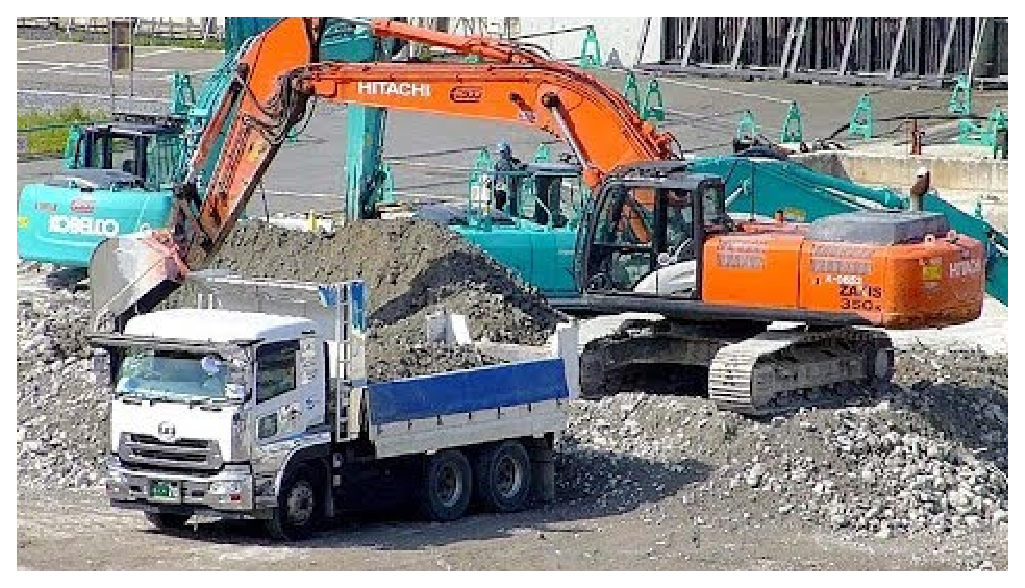
\includegraphics[width=0.8\columnwidth]{./chap1/fig/dosha.eps}
    \caption{土砂積み込み作業の様子}
    \label{fig:dosha}
    \end{center}
    %\vspace{-5mm}
\end{figure}
 
\begin{figure}[b]
 \begin{center}
 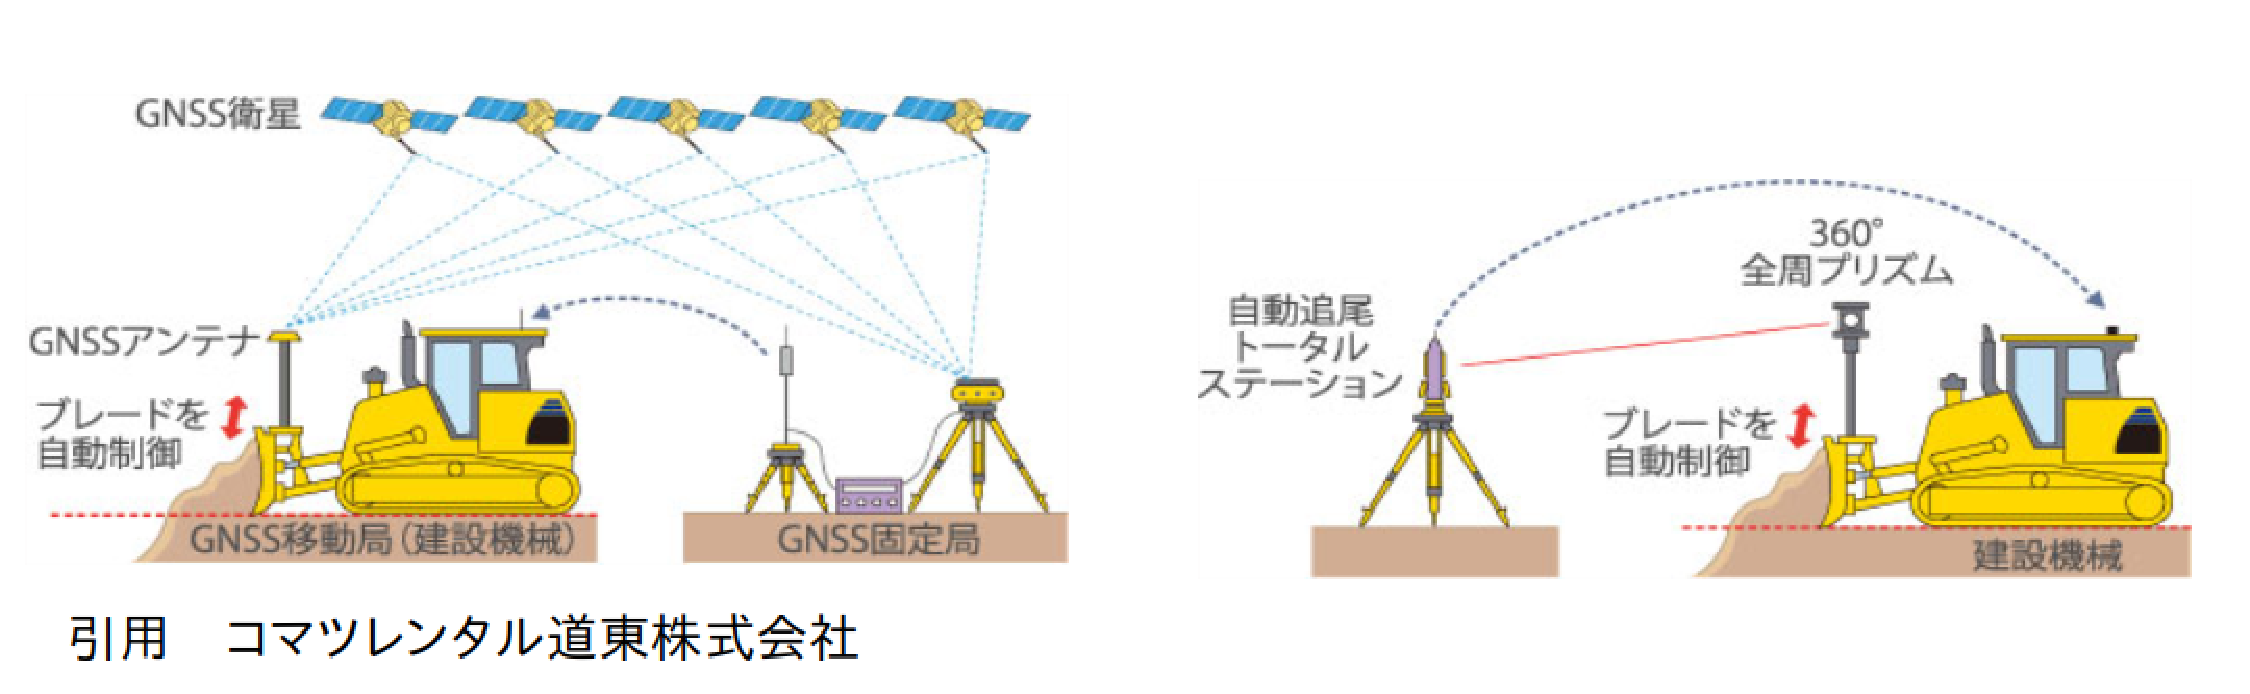
\includegraphics[width=0.8\columnwidth]{./chap1/fig/gnss.eps}
 \caption{GNSSやTSによる位置情報の把握}
 \label{fig:GNSS}
 \end{center}
 %\vspace{-5mm}
\end{figure}
%%%%%

\newpage

\section{従来研究}
車両ような移動物体に対してはロータリーエンコーダ,IMUや地磁気センサ等の移動量,姿勢,方位を計測可能なセンサを搭載による位置姿勢の計測が適している.
しかし,土砂積み込み作業では複数台のダンプトラックが入れ替わりで作業を行うため,個々にセンサ類を搭載するのは時間とコストが大きくかかる.
一方,外部からカメラや距離センサによって計測した情報を基に位置姿勢推定を行う手法が研究されており,CADモデルを用いた手法が研究されている\cite{中原智治2001}\cite{西卓郎2014}.
\par
CADモデルを用いた手法の代表例として距離センサを用いた対象物体のCADモデルとの照合による3次元物体計測がある\cite{林2008}.
この手法は,距離画像センサから計測した3次元点群と対象物体のCADモデルから作成した3次元点群を点群位置合わせすることで位置姿勢推定を行う.
また近年では深層学習を取り入れたアプローチも増えており,対象物体のあらゆる姿勢の画像をCADデータから生成したものを教師データとした深層学習による推定手法\cite{Sundermeyer2018}や,
3次元のシミュレーター環境で作成した教室データを学習することで推定する手法\cite{Tremblay2018}などが研究されている.
しかし,実際の作業現場では様々なメーカーのダンプトラックが行き交い,また荷台部も現場によって異なるため,事前にCADデータを用意するのは難しい.

\newpage

一方,車両を対象としたモデルレスの位置姿勢推定の手法としてLIDARを用いた3次元物体検出がある.\cite{Zhang2017}\cite{Chen2017}\cite{Lang2019}\\
図\ref{fig:Lidar}のように広域にレーザーを照射することにより計測した3次元点群から対象物体の点群を検出することで位置姿勢推定を行う.
しかし,土砂積み込み作業は効率的に作業を行うために高低差をつけて作業する場合が多い.そのため,LIDARは視野角が狭いため高低差があると近距離が死角になる.また,LIDARを傾けることで死角を
軽減可能だが,レーザーの密度が低いため距離によっては対象物体にレーザー当たらず計測ができない状況が生じる.
\begin{figure}[b]
    \begin{center}
    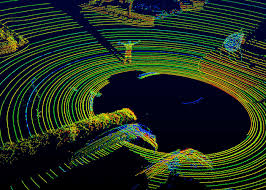
\includegraphics[width=0.8\columnwidth]{./chap1/fig/lidar.eps}
    \caption{Lidarによる計測データ}
    \label{fig:Lidar}
    \end{center}
\end{figure}


\newpage
\section{研究の目的}
1.1 節で述べたように,環境に大がかりな設備を要せずにダンプトラックの位置姿勢を計測する手法が求められている.
そのための計測方法として距離画像センサの計測データとCADモデルを用いた位置姿勢推定が有効である.
しかし,CADモデルを用いた手法は事前にCADモデルを用意する必要があり,作業現場では用意が難しいという問題がある.
また,距離画像センサは点群位置合わせを行う上で有効な高密度の3次元点群を得られるが,計測距離が短く計測できる範囲は土砂積み込み作業が可能な範囲であり,
土砂積み込み作業の際は,ダンプトラックは遠方からバックホウに向かって進入してくる場合が多く,ダンプトラックの進入を判断するためには,
遠方にあるダンプトラックの存在とその大まかな位置姿勢を計測する必要がある.
そのため,RGB-Dセンサの有効範囲に依存しない位置姿勢推定手法が必要である.



\par
そこで,本研究では
    \begin{screen}
        \begin{center}
            画像による3次元物体検出と\\点群位置合わせによる位置姿勢推定の手法を提案
        \end{center}
    \end{screen}
を目的とする
\newpage
\section{本論文の構成}
本論文は全4章から構成されている.図\ref{fig:GNSS}に本論文の構成を示す.\par
第1章では,本研究の背景,従来研究,目的について述べた.\par
第2章では,画像認識と点群位置合わせによるダンプトラックの位置姿勢推定の提案手法について述べる.\par
第3章では,本提案手法の有効性を検証するために行った実験について述べる.\par
第4章では,結論と今後の展望を述べる.
\begin{figure}[b]
    \begin{center}
    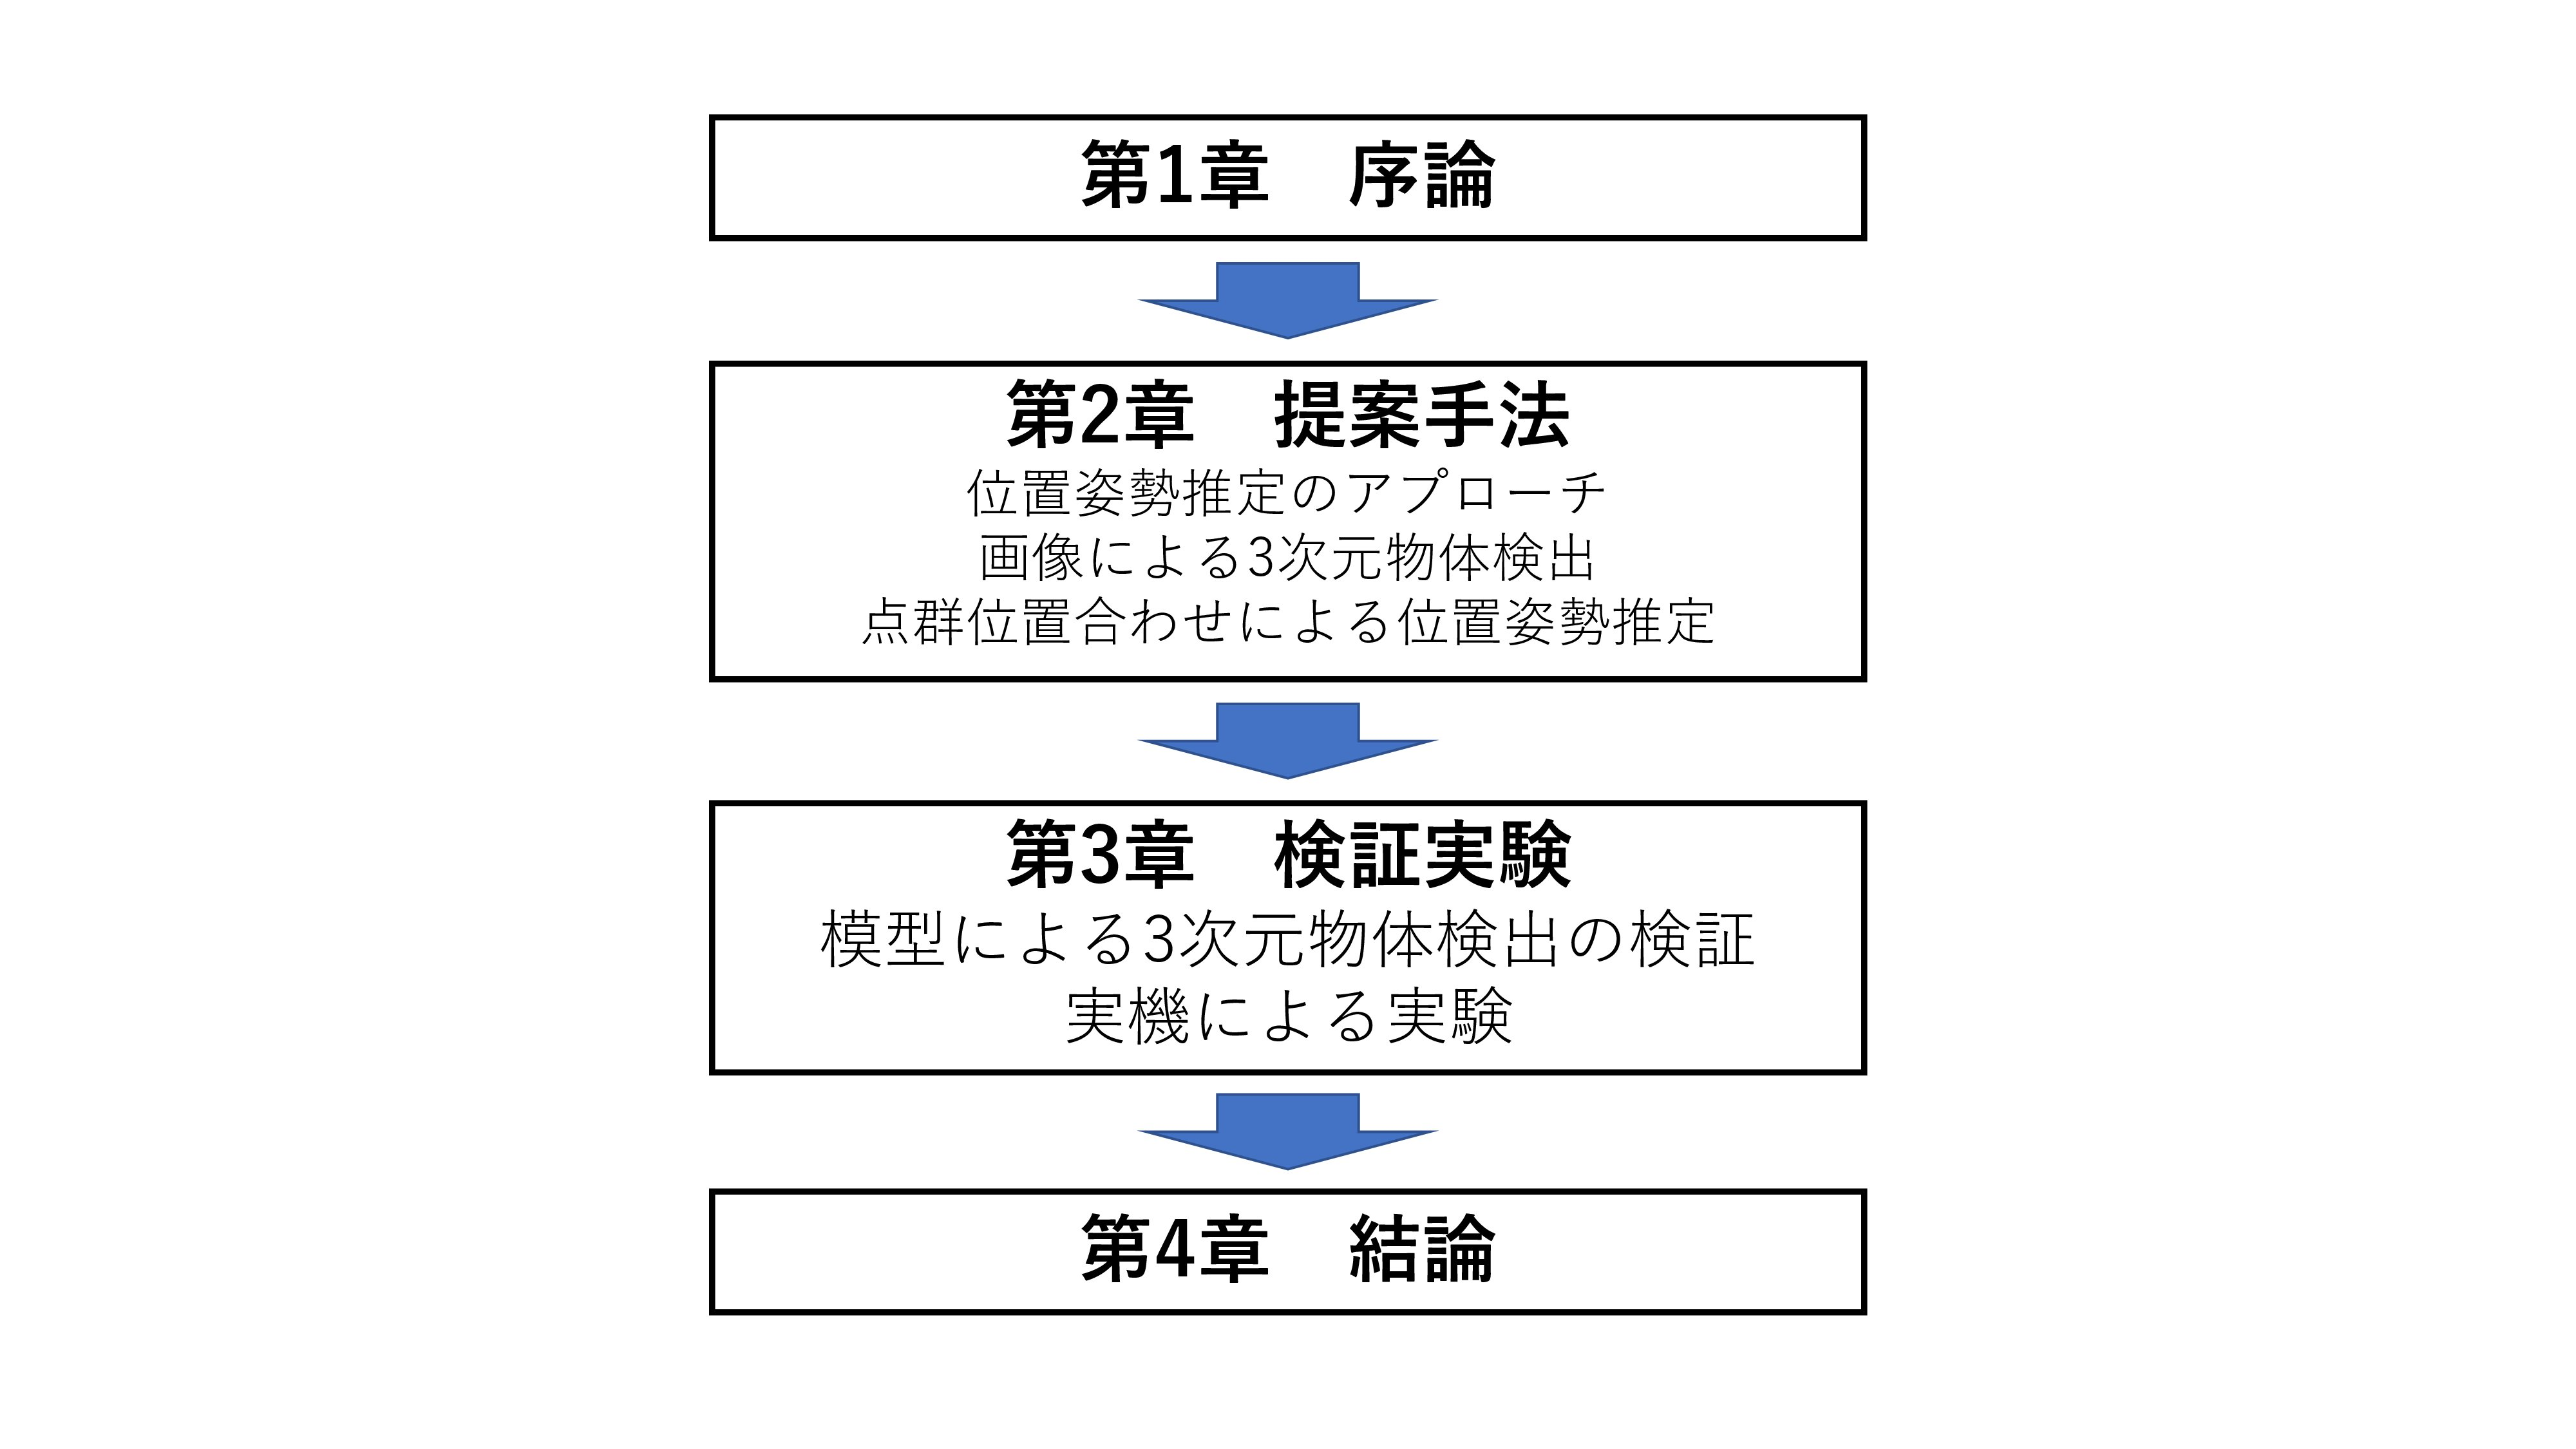
\includegraphics[width=1.0 \columnwidth]{./chap1/fig/struct.eps}
    \caption{本論文の構成}
    \label{fig:flow}
    \end{center}
    %\vspace{-5mm}
\end{figure}

%%%%%%%%%%%%%%%%%%%%%%%%%%%%%%%%%%%%%%%%%%%%%%%%%%%%%%%%%%%%%%%%%%%%%%%%%%%%%%%
%%% Local Variables:
%%% mode: katex
%%% TeX-master: "../thesis"
%%% End: